% 由 tools/md2tex.py 自 2023_数学真题_试题.md 生成，勿手改（改源 MD 后重跑）


\begin{gknotice}
\textbf{结构提示}：本卷为 \textbf{22 题制}（多选 4 题、填空 4 题、解答 6 题）。2024 年起新高考 I 卷改为 19 题制，故本卷\textbf{不宜整套限时模拟}，建议按知识点抽题使用。

\textbf{适用省份}：山东、广东、湖南、湖北、河北、江苏、福建、浙江
\end{gknotice}

\par\medskip

\gkpart{一、单选题}

\begin{gktip}
本题共 8 小题，每小题 5 分，共 40 分。在每小题给出的四个选项中，只有一项是符合题目要求的。
\end{gktip}

\gkti{1}已知集合 $M=\{-2,-1,0,1,2\}$，$N=\left\{x\mid x^{2}-x-6\ge0\right\}$，则 $M\cap N=$（　　）

\begin{gkopts}(4)
\task A．$\{-2,-1,0,1\}$
\task B．$\{0,1,2\}$
\task C．$\{-2\}$
\task D．$\{2\}$
\end{gkopts}

\gkti{2}已知 $z=\dfrac{1-\mathrm i}{2+2\mathrm i}$，则 $z-\bar z=$（　　）

\begin{gkopts}(4)
\task A．$-\mathrm i$
\task B．$\mathrm i$
\task C．$0$
\task D．$1$
\end{gkopts}

\gkti{3}已知向量 $\boldsymbol a=(1,1)$，$\boldsymbol b=(1,-1)$。若 $(\boldsymbol a+\lambda\boldsymbol b)\perp(\boldsymbol a+\mu\boldsymbol b)$，则（　　）

\begin{gkopts}(4)
\task A．$\lambda+\mu=1$
\task B．$\lambda+\mu=-1$
\task C．$\lambda\mu=1$
\task D．$\lambda\mu=-1$
\end{gkopts}

\gkti{4}设函数 $f(x)=2^{x(x-a)}$ 在区间 $(0,1)$ 单调递减，则 $a$ 的取值范围是（　　）

\begin{gkopts}(4)
\task A．$(-\infty,-2]$
\task B．$[-2,0)$
\task C．$(0,2]$
\task D．$[2,+\infty)$
\end{gkopts}

\gkti{5}设椭圆 $C_1:\dfrac{x^{2}}{a^{2}}+y^{2}=1\ (a>1)$，$C_2:\dfrac{x^{2}}4+y^{2}=1$ 的离心率分别为 $e_1$，$e_2$。若 $e_2=\sqrt3\,e_1$，则 $a=$（　　）

\begin{gkopts}(2)
\task A．$\dfrac{2\sqrt3}3$
\task B．$\sqrt2$
\task C．$\sqrt3$
\task D．$\sqrt6$
\end{gkopts}

\gkti{6}过点 $(0,-2)$ 与圆 $x^{2}+y^{2}-4x-1=0$ 相切的两条直线的夹角为 $\alpha$，则 $\sin\alpha=$（　　）

\begin{gkopts}(2)
\task A．$1$
\task B．$\dfrac{\sqrt{15}}4$
\task C．$\dfrac{\sqrt{10}}4$
\task D．$\dfrac{\sqrt6}4$
\end{gkopts}

\gkti{7}记 $S_n$ 为数列 $\left\{a_n\right\}$ 的前 $n$ 项和，设甲：$\left\{a_n\right\}$ 为等差数列；乙：$\left\{\dfrac{S_n}n\right\}$ 为等差数列，则（　　）

\begin{gkopts}(2)
\task A．甲是乙的充分条件但不是必要条件
\task B．甲是乙的必要条件但不是充分条件
\task C．甲是乙的充要条件
\task D．甲既不是乙的充分条件也不是乙的必要条件
\end{gkopts}

\gkti{8}已知 $\sin(\alpha-\beta)=\dfrac13$，$\cos\alpha\sin\beta=\dfrac16$，则 $\cos(2\alpha+2\beta)=$（　　）

\begin{gkopts}(4)
\task A．$\dfrac79$
\task B．$\dfrac19$
\task C．$-\dfrac19$
\task D．$-\dfrac79$
\end{gkopts}

\par\medskip

\gkpart{二、多选题}

\begin{gktip}
本题共 4 小题，每小题 5 分，共 20 分。全部选对得 5 分，部分选对得 2 分，有选错得 0 分。
\end{gktip}

\gkti{9}有一组样本数据 $x_1,x_2,\cdots,x_6$，其中 $x_1$ 是最小值，$x_6$ 是最大值，则（　　）

\begin{gkopts}(1)
\task A．$x_2,x_3,x_4,x_5$ 的平均数等于 $x_1,x_2,\cdots,x_6$ 的平均数
\task B．$x_2,x_3,x_4,x_5$ 的中位数等于 $x_1,x_2,\cdots,x_6$ 的中位数
\task C．$x_2,x_3,x_4,x_5$ 的标准差不小于 $x_1,x_2,\cdots,x_6$ 的标准差
\task D．$x_2,x_3,x_4,x_5$ 的极差不大于 $x_1,x_2,\cdots,x_6$ 的极差
\end{gkopts}

\gkti{10}噪声污染问题越来越受到重视。用声压级来度量声音的强弱，定义声压级 $L_P=20\times\lg\dfrac p{p_0}$，其中常数 $p_0\ (p_0>0)$ 是听觉下限阈值，$p$ 是实际声压。下表为不同声源的声压级：

\begin{center}
\begin{tabular}{ccc}
\toprule
声源 & 与声源的距离 $/\mathrm m$ & 声压级 $/\mathrm{dB}$ \\
\midrule
燃油汽车 & $10$ & $60\sim90$ \\
混合动力汽车 & $10$ & $50\sim60$ \\
电动汽车 & $10$ & $40$ \\
\bottomrule
\end{tabular}
\end{center}

已知在距离燃油汽车、混合动力汽车、电动汽车 $10\ \mathrm m$ 处测得实际声压分别为 $p_1$，$p_2$，$p_3$，则（　　）

\begin{gkopts}(4)
\task A．$p_1\ge p_2$
\task B．$p_2>10p_3$
\task C．$p_3=100p_0$
\task D．$p_1\le100p_2$
\end{gkopts}

\gkti{11}已知函数 $f(x)$ 的定义域为 $\mathbf R$，$f(xy)=y^{2}f(x)+x^{2}f(y)$，则（　　）

\begin{gkopts}(2)
\task A．$f(0)=0$
\task B．$f(1)=0$
\task C．$f(x)$ 是偶函数
\task D．$x=0$ 为 $f(x)$ 的极小值点
\end{gkopts}

\gkti{12}下列物体中，能被整体放入棱长为 $1$（单位：$\mathrm m$）的正方体容器（容器壁厚度忽略不计）内的有（　　）

\begin{gkopts}(1)
\task A．直径为 $0.99\ \mathrm m$ 的球体
\task B．所有棱长均为 $1.4\ \mathrm m$ 的四面体
\task C．底面直径为 $0.01\ \mathrm m$，高为 $1.8\ \mathrm m$ 的圆柱体
\task D．底面直径为 $1.2\ \mathrm m$，高为 $0.01\ \mathrm m$ 的圆柱体
\end{gkopts}

\par\medskip

\gkpart{三、填空题}

\begin{gktip}
本题共 4 小题，每小题 5 分，共 20 分。
\end{gktip}

\gkti{13}某学校开设了 $4$ 门体育类选修课和 $4$ 门艺术类选修课，学生需从这 $8$ 门课中选修 $2$ 门或 $3$ 门，并且每类选修课至少选修 $1$ 门，则不同的选课方案共有 \gkblank{} 种（用数字作答）。

\gkti{14}在正四棱台 $ABCD\text{-}A_1B_1C_1D_1$ 中，$AB=2$，$A_1B_1=1$，$AA_1=\sqrt2$，则该棱台的体积为 \gkblank{}．

\gkti{15}已知函数 $f(x)=\cos\omega x-1\ (\omega>0)$ 在区间 $[0,2\pi]$ 有且仅有 $3$ 个零点，则 $\omega$ 的取值范围是 \gkblank{}．

\gkti{16}已知双曲线 $C:\dfrac{x^{2}}{a^{2}}-\dfrac{y^{2}}{b^{2}}=1\ (a>0,\ b>0)$ 的左、右焦点分别为 $F_1$，$F_2$。点 $A$ 在 $C$ 上，点 $B$ 在 $y$ 轴上，$\overrightarrow{F_1A}\perp\overrightarrow{F_1B}$，$\overrightarrow{F_2A}=-\dfrac23\overrightarrow{F_2B}$，则 $C$ 的离心率为 \gkblank{}．

\par\medskip

\gkpart{四、解答题}

\begin{gktip}
本题共 6 小题，共 70 分。解答应写出文字说明、证明过程或演算步骤。
\end{gktip}

\gkti{17}\textbf{（10 分）} 已知在 $\triangle ABC$ 中，$A+B=3C$，$2\sin(A-C)=\sin B$。

  (1) 求 $\sin A$；

  (2) 设 $AB=5$，求 $AB$ 边上的高。

\gkti{18}\textbf{（12 分）} 如图，在正四棱柱 $ABCD\text{-}A_1B_1C_1D_1$ 中，$AB=2$，$AA_1=4$。点 $A_2$，$B_2$，$C_2$，$D_2$ 分别在棱 $AA_1$，$BB_1$，$CC_1$，$DD_1$ 上，$AA_2=1$，$BB_2=DD_2=2$，$CC_2=3$。

\begin{center}% 2023 新高考Ⅰ卷 18：正四棱柱 ABCD-A1B1C1D1，A2/B2/C2/D2 分别在四条侧棱上
% （AA2=1、BB2=DD2=2、CC2=3），P 在棱 BB1 上
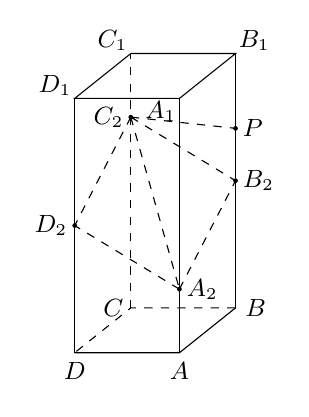
\begin{tikzpicture}[scale=0.95, font=\small]
  \coordinate (D)  at (0,0);
  \coordinate (A)  at (1.4,0);
  \coordinate (B)  at (2.15,0.6);
  \coordinate (C)  at (0.75,0.6);
  \coordinate (D1) at (0,3.4);
  \coordinate (A1) at (1.4,3.4);
  \coordinate (B1) at (2.15,4.0);
  \coordinate (C1) at (0.75,4.0);
  \coordinate (A2) at (1.4,0.85);
  \coordinate (B2) at (2.15,2.3);
  \coordinate (C2) at (0.75,3.15);
  \coordinate (D2) at (0,1.7);
  \coordinate (P)  at (2.15,3.0);
  \draw (D) -- (A) -- (B);
  \draw[dashed] (B) -- (C) -- (D);
  \draw (D) -- (D1)  (A) -- (A1)  (B) -- (B1);
  \draw[dashed] (C) -- (C1);
  \draw (D1) -- (A1) -- (B1) -- (C1) -- cycle;
  \draw[dashed] (C2) -- (A2)  (C2) -- (B2)  (C2) -- (D2)  (C2) -- (P);
  \draw[dashed] (A2) -- (B2)  (A2) -- (D2);
  \fill (A2) circle (0.9pt); \fill (B2) circle (0.9pt);
  \fill (C2) circle (0.9pt); \fill (D2) circle (0.9pt); \fill (P) circle (0.9pt);
  \node[below] at (D) {$D$};
  \node[below] at (A) {$A$};
  \node[right] at (B) {$B$};
  \node[left, inner sep=2.5pt] at (C) {$C$};
  \node[above left, inner sep=1pt] at (D1) {$D_1$};
  \node[below left, inner sep=1pt] at (A1) {$A_1$};
  \node[above right, inner sep=1pt] at (B1) {$B_1$};
  \node[above left, inner sep=1pt] at (C1) {$C_1$};
  \node[right, inner sep=2.5pt] at (A2) {$A_2$};
  \node[right, inner sep=2.5pt] at (B2) {$B_2$};
  \node[left, inner sep=2.5pt] at (C2) {$C_2$};
  \node[left, inner sep=2.5pt] at (D2) {$D_2$};
  \node[right, inner sep=2.5pt] at (P) {$P$};
\end{tikzpicture}
\end{center}

  (1) 证明：$B_2C_2\parallel A_2D_2$；

  (2) 点 $P$ 在棱 $BB_1$ 上，当二面角 $P\text{-}A_2C_2\text{-}D_2$ 为 $150^\circ$ 时，求 $B_2P$。

\gkti{19}\textbf{（12 分）} 已知函数 $f(x)=a\left(\mathrm e^{x}+a\right)-x$。

  (1) 讨论 $f(x)$ 的单调性；

  (2) 证明：当 $a>0$ 时，$f(x)>2\ln a+\dfrac32$。

\gkti{20}\textbf{（12 分）} 设等差数列 $\left\{a_n\right\}$ 的公差为 $d$，且 $d>1$。令 $b_n=\dfrac{n^{2}+n}{a_n}$，记 $S_n$，$T_n$ 分别为数列 $\left\{a_n\right\}$，$\left\{b_n\right\}$ 的前 $n$ 项和。

  (1) 若 $3a_2=3a_1+a_3$，$S_3+T_3=21$，求 $\left\{a_n\right\}$ 的通项公式；

  (2) 若 $\left\{b_n\right\}$ 为等差数列，且 $S_{99}-T_{99}=99$，求 $d$。

\gkti{21}\textbf{（12 分）} 甲、乙两人投篮，每次由其中一人投篮，规则如下：若命中则此人继续投篮，若未命中则换为对方投篮。无论之前投篮情况如何，甲每次投篮的命中率均为 $0.6$，乙每次投篮的命中率均为 $0.8$。由抽签决定第 $1$ 次投篮的人选，第 $1$ 次投篮的人是甲、乙的概率各为 $0.5$。

  (1) 求第 $2$ 次投篮的人是乙的概率；

  (2) 求第 $i$ 次投篮的人是甲的概率；

  (3) 已知：若随机变量 $X_i$ 服从两点分布，且 $P\left(X_i=1\right)=1-P\left(X_i=0\right)=q_i$，$i=1,2,\cdots,n$，则 $E\left(\displaystyle\sum_{i=1}^{n}X_i\right)=\displaystyle\sum_{i=1}^{n}q_i$。记前 $n$ 次（即从第 $1$ 次到第 $n$ 次投篮）中甲投篮的次数为 $Y$，求 $E(Y)$。

\gkti{22}\textbf{（12 分）} 在直角坐标系 $xOy$ 中，点 $P$ 到 $x$ 轴的距离等于点 $P$ 到点 $\left(0,\dfrac12\right)$ 的距离，记动点 $P$ 的轨迹为 $W$。

  (1) 求 $W$ 的方程；

  (2) 已知矩形 $ABCD$ 有三个顶点在 $W$ 上，证明：矩形 $ABCD$ 的周长大于 $3\sqrt3$。

\par\medskip

